\section{Numerical results}
\begin{itemize}
    \item Introduce example problem (target = sol to forward/primal eqn with a known source/forcing $g$)
    \item Convergence plots (both "iterative" error $u^{(k)} - u^{(k-1)}$ and "absolute" error $u^{(k)}-u^{(*)}$)
    \item Plots showing comparison of target sol and actual obtained sol (snapshots in time) ((Maybe not))
    \item Example sol of forward equation using Monte Carlo
    \item Example sol of backward equation? Maybe.
\end{itemize}

\subsection{Setting for numerical results}
For the purposes of numerical simulations, we consider a simple Gaussian target radiation intensity given by
%
\begin{align}
    d_T(t,x,v) = \exp\Big[ -c\big( {(x-e)}^2 + {(v-d)}^2 \big) \Big].
\end{align}
%

%
\begin{align}
    f_0(x,v) = \exp\Big[ -c\big( {(x-e)}^2 + {(v-d)}^2 \big) \Big]
\end{align}
%

\begin{figure}[h]
    \centering
    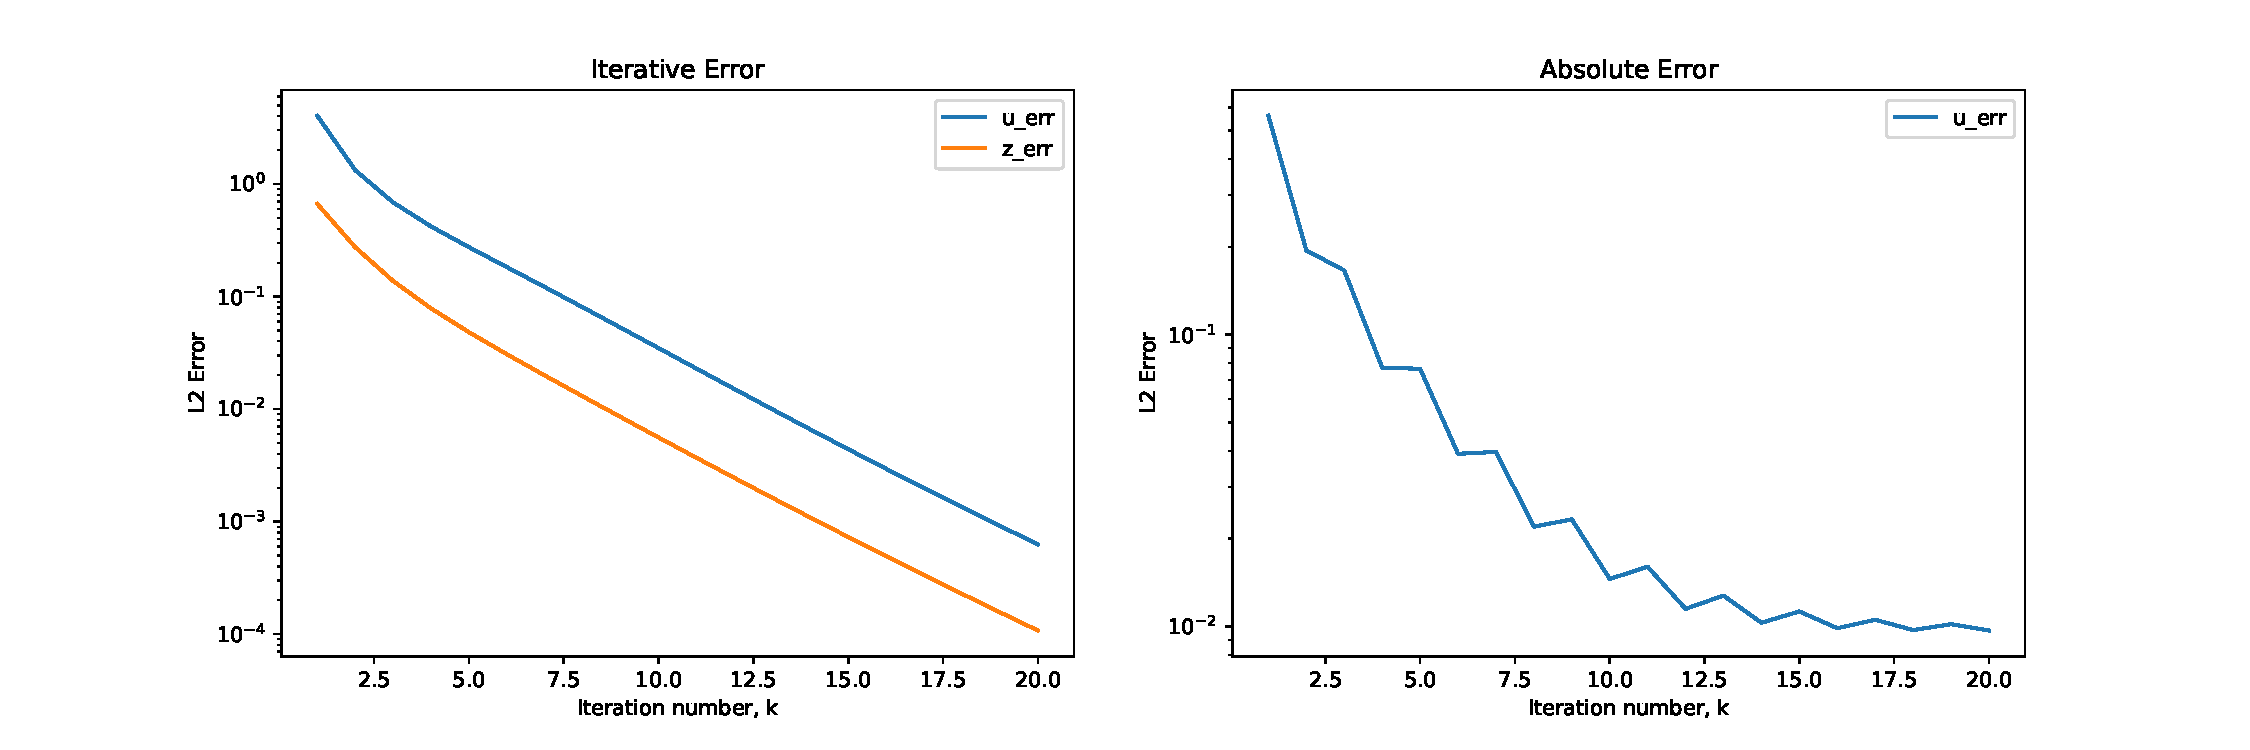
\includegraphics[width=0.9\textwidth]{error_plots.pdf}
    \caption{Error plots.}\label{fig:error-plots}
\end{figure}
